\clearpage
\section{Problembeskrivelse}
\label{problemBeskrivelse}


%Her kan du skrive om din problembeskrivelse
I dette designotatet skal det designes to ting som tilsammen vil utføre en oppgave. Oppgaven er å filtrere frem en spesifik tone ut av hvit støy. De to delene som skal designes er en hvit støy generator og et aktivt filter. Hvit støy generatoren skla designes ved hjelp av en FPGA og skal generere hvit støy som skal mates inn i det aktive filteret. Det aktive filteret vil filtrere ut støyen så det kun er en spesifikk tone igjen. Denne tonen skal så kunne spilles av på en høyttaler eller PC.I figur \ref{overview} er det vist en oversikt over hvordan sluttsystemet kan se ut.

\begin{figure}[!h]
\centering
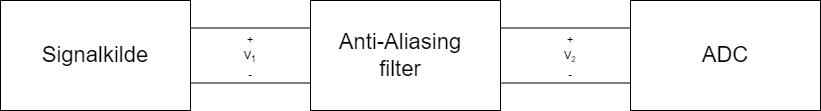
\includegraphics[width=1\linewidth]{Bilder/overblikk.drawio.png}
\caption{Sluttsystemet kan se ut som dette}
\label{overview}
\end{figure}